\documentclass{article}[12pt]

% General packages
\usepackage[english]{babel}
\pagenumbering{arabic}
\usepackage{color}
\usepackage{lettrine}
\usepackage{setspace}
\usepackage{yfonts}
\usepackage{type1cm}


% Graphics packages
\usepackage{graphicx}
\usepackage{rotating}


% Math packages
\usepackage{array}
\usepackage{amsmath}
\usepackage{amsfonts}
\usepackage{amssymb}
\usepackage{geometry}
\usepackage{xparse}
\usepackage{physics}

% Links packages
\usepackage{hyperref}
\usepackage{url}
\usepackage{xcolor}
\hypersetup{
    colorlinks,
    linkcolor={blue!80!black},
    citecolor={blue!80!black},
    urlcolor={blue!80!black}
}


% Tables packages
\usepackage{adjustbox}
\usepackage{multirow}
\usepackage{hhline}
\usepackage{float}
\usepackage[bottom]{footmisc}
\usepackage{booktabs,caption}
\usepackage[flushleft]{threeparttable}
\usepackage[labelfont=sc]{caption}
\captionsetup[table]{skip=0pt}


% citations
\usepackage[round]{natbib}   % omit 'round' option if you prefer square brackets
%\bibliographystyle{plainnat}
%\bibliographystyle{abbrv}
%\bibliographystyle{acm}
%\bibliographystyle{alpha}
\bibliographystyle{apalike}
%\bibliographystyle{ieeetr}
%\bibliographystyle{plain}
%\bibliographystyle{siam}
%\bibliographystyle{unsrt}

% figures
\usepackage{subcaption}


\begin{document}

\title{Problem Set 8}
\author{Angela Shoulders}
\date{December 3, 2021}

\maketitle

The model I have created is an individual model for health and health related activities.  All of us are aware, even if it's just in a philisophical sense, that our actions every day have an impact on our health in the future.  Fortunately (or perhaps unfortunately), our body takes a long time to incorporate the small health related decisions we make every day.  This is why we don't see the benefits of our good choices immediately, and conversely we don't deal with the consequenses of our bad choices when we make them.  This model attempts to show this concept.

\begin{enumerate}
    \item Population of agents
    \begin{itemize}
        \item We are modeling inidvidual decisions for health and health related activities
    \end{itemize}
    \item Preferences
    \begin{itemize}
        \item Our utility function is increasing and concave.  Our individuals get utility from their health in the current period, $h_t$, and from the negative health choices we make (e.g. eating brownies), $c_t$.  Note that a negative value of $c$ refers to a good choice and a positive value of $c$ refers to a bad choice.  This is counterintuitive but it's the best way I could make the problem work.
        \item The actual utility function is $u(h, c) = h ^ \phi + \omega  c$
        \item We have a discount factor $\beta$ which is between 0 and 1.  This discount factor disounts our future utility.
        \item We have a second disount factor $\delta$, also between 0 and 1.  This discount factor dampens the positive effects of our good health behaviour and the negative effects of our bad health behaviour.
    \end{itemize}
    \item Productive technology
    \begin{itemize}
        \item In the initial period, the individual is given an elotment of health, $h_1 > 0$.  This helps represent the baseline differences in people's health.  Some people are born with a higher baseline of heatlh (and thus have a higher $h_1$), whereas others are born with chronic health conditions (and thus have a lower $h_1$).
        \item Health is subject to the following equation : $h_{t+1} = h_t - \delta c_t$.  This means that the individual's health tomorrow is based on their health today plus the discounted health choices they make today.  Their health choices, $c_t$, can be healthy (though negative in sign) or unhealthy (though positive in sign).
        \item Note: Health can never be negative.  In all periods, health must be greater than or equal to 0.
    \end{itemize}
    \item Information technology
    \begin{itemize}
        \item The individual has perfect information and knows both the magnitude and direction of the health choices they make in each period.
    \end{itemize}
    \item Enforcement technology
    \begin{itemize}
        \item N/A
    \end{itemize}
    \item Matching technology
    \begin{itemize}
        \item N/A
    \end{itemize}
    \item The state variable is $h_1$ and the control variables are $c_t$ and $h_{t+1}$
\end{enumerate}

Our problem is:

\begin{equation}
\begin{aligned}
    \label{eq:max}
    \min_{c_t, h_{t+1}} \sum_{t=1}^\infty \beta^{t-1} h_t ^ \phi + \omega c_t \\
    \textrm{s.t.} \ i) \ h_{t+1} = h_t - \delta c_t \\
    ii) \ h_1 > 0 \ given \\
    iii) \ c_t \neq 0 \\
    iv) \ u' > 0, u'' < 0 , u'(0) = \infty, u'(\infty) = 0
\end{aligned}
\end{equation}

This implies our Lagrangian:
\begin{equation}
\begin{aligned}
    \label{eq:lagrangian}
    \mathcal{L} = \sum_{t=1}^\infty \beta^{t-1} [h_t ^ \phi + \omega c_t] +  \lambda_t \sum_{t=1}^\infty [h_{t+1} - h_t + \delta c_t]
\end{aligned}
\end{equation}

FOCs:

\begin{equation}
\begin{aligned}
    \label{eq:fonc}
    \frac{\partial \mathcal{L}}{\partial h_{t+1}} = \lambda_t + \beta ^t \phi h_{t+1} ^ {\phi - 1} - \lambda_{t+1} = 0 \\
    \frac{\partial \mathcal{L}}{\partial c_t} = \beta ^ {t-1} \omega + \lambda_t \delta  = 0 \\
\end{aligned}
\end{equation}

The Bellman equation is:

\begin{equation}
\begin{aligned}
    \label{eq:bellman}
    v_{T+1}(h_1) = u(h_1) + \beta v_T (h_{T+1})
\end{aligned}
\end{equation}

\pagebreak

I solved and plotted this problem in python (see execute.py and functions.py for details).  Below is the plotted value function.  Unsurprisingly, as a person accumulates more health (either by starting at a higher level of health or by engaginge in heatlthy activities), their value goes up.

\begin{figure}[h]
    \centering
    \caption{\textsc{Value Function}}
    \label{fig:plot1}
    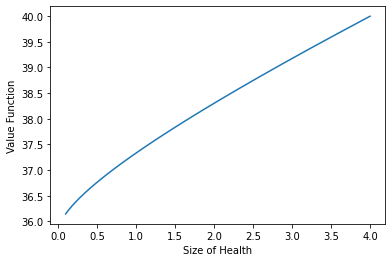
\includegraphics[scale=0.6]{plot1.png}
    \hspace{0.5cm}
\end{figure}

\end{document}